\documentclass[1p]{elsarticle_modified}
%\bibliographystyle{elsarticle-num}

%\usepackage[colorlinks]{hyperref}
%\usepackage{abbrmath_seonhwa} %\Abb, \Ascr, \Acal ,\Abf, \Afrak
\usepackage{amsfonts}
\usepackage{amssymb}
\usepackage{amsmath}
\usepackage{amsthm}
\usepackage{scalefnt}
\usepackage{amsbsy}
\usepackage{kotex}
\usepackage{caption}
\usepackage{subfig}
\usepackage{color}
\usepackage{graphicx}
\usepackage{xcolor} %% white, black, red, green, blue, cyan, magenta, yellow
\usepackage{float}
\usepackage{setspace}
\usepackage{hyperref}

\usepackage{tikz}
\usetikzlibrary{arrows}

\usepackage{multirow}
\usepackage{array} % fixed length table
\usepackage{hhline}

%%%%%%%%%%%%%%%%%%%%%
\makeatletter
\renewcommand*\env@matrix[1][\arraystretch]{%
	\edef\arraystretch{#1}%
	\hskip -\arraycolsep
	\let\@ifnextchar\new@ifnextchar
	\array{*\c@MaxMatrixCols c}}
\makeatother %https://tex.stackexchange.com/questions/14071/how-can-i-increase-the-line-spacing-in-a-matrix
%%%%%%%%%%%%%%%

\usepackage[normalem]{ulem}

\newcommand{\msout}[1]{\ifmmode\text{\sout{\ensuremath{#1}}}\else\sout{#1}\fi}
%SOURCE: \msout is \stkout macro in https://tex.stackexchange.com/questions/20609/strikeout-in-math-mode

\newcommand{\cancel}[1]{
	\ifmmode
	{\color{red}\msout{#1}}
	\else
	{\color{red}\sout{#1}}
	\fi
}

\newcommand{\add}[1]{
	{\color{blue}\uwave{#1}}
}

\newcommand{\replace}[2]{
	\ifmmode
	{\color{red}\msout{#1}}{\color{blue}\uwave{#2}}
	\else
	{\color{red}\sout{#1}}{\color{blue}\uwave{#2}}
	\fi
}

\newcommand{\Sol}{\mathcal{S}} %segment
\newcommand{\D}{D} %diagram
\newcommand{\A}{\mathcal{A}} %arc


%%%%%%%%%%%%%%%%%%%%%%%%%%%%%5 test

\def\sl{\operatorname{\textup{SL}}(2,\Cbb)}
\def\psl{\operatorname{\textup{PSL}}(2,\Cbb)}
\def\quan{\mkern 1mu \triangleright \mkern 1mu}

\theoremstyle{definition}
\newtheorem{thm}{Theorem}[section]
\newtheorem{prop}[thm]{Proposition}
\newtheorem{lem}[thm]{Lemma}
\newtheorem{ques}[thm]{Question}
\newtheorem{cor}[thm]{Corollary}
\newtheorem{defn}[thm]{Definition}
\newtheorem{exam}[thm]{Example}
\newtheorem{rmk}[thm]{Remark}
\newtheorem{alg}[thm]{Algorithm}

\newcommand{\I}{\sqrt{-1}}
\begin{document}

%\begin{frontmatter}
%
%\title{Boundary parabolic representations of knots up to 8 crossings}
%
%%% Group authors per affiliation:
%\author{Yunhi Cho} 
%\address{Department of Mathematics, University of Seoul, Seoul, Korea}
%\ead{yhcho@uos.ac.kr}
%
%
%\author{Seonhwa Kim} %\fnref{s_kim}}
%\address{Center for Geometry and Physics, Institute for Basic Science, Pohang, 37673, Korea}
%\ead{ryeona17@ibs.re.kr}
%
%\author{Hyuk Kim}
%\address{Department of Mathematical Sciences, Seoul National University, Seoul 08826, Korea}
%\ead{hyukkim@snu.ac.kr}
%
%\author{Seokbeom Yoon}
%\address{Department of Mathematical Sciences, Seoul National University, Seoul, 08826,  Korea}
%\ead{sbyoon15@snu.ac.kr}
%
%\begin{abstract}
%We find all boundary parabolic representation of knots up to 8 crossings.
%
%\end{abstract}
%\begin{keyword}
%    \MSC[2010] 57M25 
%\end{keyword}
%
%\end{frontmatter}

%\linenumbers
%\tableofcontents
%
\newcommand\colored[1]{\textcolor{white}{\rule[-0.35ex]{0.8em}{1.4ex}}\kern-0.8em\color{red} #1}%
%\newcommand\colored[1]{\textcolor{white}{ #1}\kern-2.17ex	\textcolor{white}{ #1}\kern-1.81ex	\textcolor{white}{ #1}\kern-2.15ex\color{red}#1	}

{\Large $\underline{12n_{0826}~(K12n_{0826})}$}

\setlength{\tabcolsep}{10pt}
\renewcommand{\arraystretch}{1.6}
\vspace{1cm}\begin{tabular}{m{100pt}>{\centering\arraybackslash}m{274pt}}
\multirow{5}{120pt}{
	\centering
	\includegraphics[width=112pt]{../../../GIT/diagram.site/Diagrams/png/2915_12n_0826.png}\\
\ \ \ A knot diagram\footnotemark}&
\allowdisplaybreaks
\textbf{Linearized knot diagam} \\
\cline{2-2}
 &
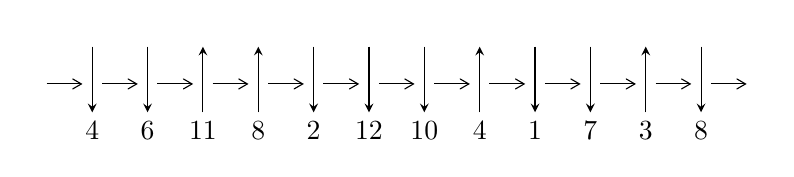
\begin{tikzpicture}[x=20pt, y=17pt]
	% nodes
	\node (C0) at (0, 0) {};
	\node (C1) at (1, 0) {};
	\node (C1U) at (1, +1) {};
	\node (C1D) at (1, -1) {4};

	\node (C2) at (2, 0) {};
	\node (C2U) at (2, +1) {};
	\node (C2D) at (2, -1) {6};

	\node (C3) at (3, 0) {};
	\node (C3U) at (3, +1) {};
	\node (C3D) at (3, -1) {11};

	\node (C4) at (4, 0) {};
	\node (C4U) at (4, +1) {};
	\node (C4D) at (4, -1) {8};

	\node (C5) at (5, 0) {};
	\node (C5U) at (5, +1) {};
	\node (C5D) at (5, -1) {2};

	\node (C6) at (6, 0) {};
	\node (C6U) at (6, +1) {};
	\node (C6D) at (6, -1) {12};

	\node (C7) at (7, 0) {};
	\node (C7U) at (7, +1) {};
	\node (C7D) at (7, -1) {10};

	\node (C8) at (8, 0) {};
	\node (C8U) at (8, +1) {};
	\node (C8D) at (8, -1) {4};

	\node (C9) at (9, 0) {};
	\node (C9U) at (9, +1) {};
	\node (C9D) at (9, -1) {1};

	\node (C10) at (10, 0) {};
	\node (C10U) at (10, +1) {};
	\node (C10D) at (10, -1) {7};

	\node (C11) at (11, 0) {};
	\node (C11U) at (11, +1) {};
	\node (C11D) at (11, -1) {3};

	\node (C12) at (12, 0) {};
	\node (C12U) at (12, +1) {};
	\node (C12D) at (12, -1) {8};
	\node (C13) at (13, 0) {};

	% arrows
	\draw[->,>={angle 60}]
	(C0) edge (C1) (C1) edge (C2) (C2) edge (C3) (C3) edge (C4) (C4) edge (C5) (C5) edge (C6) (C6) edge (C7) (C7) edge (C8) (C8) edge (C9) (C9) edge (C10) (C10) edge (C11) (C11) edge (C12) (C12) edge (C13) ;	\draw[->,>=stealth]
	(C1U) edge (C1D) (C2U) edge (C2D) (C3D) edge (C3U) (C4D) edge (C4U) (C5U) edge (C5D) (C6U) edge (C6D) (C7U) edge (C7D) (C8D) edge (C8U) (C9U) edge (C9D) (C10U) edge (C10D) (C11D) edge (C11U) (C12U) edge (C12D) ;
	\end{tikzpicture} \\
\hhline{~~} \\& 
\textbf{Solving Sequence} \\ \cline{2-2} 
 &
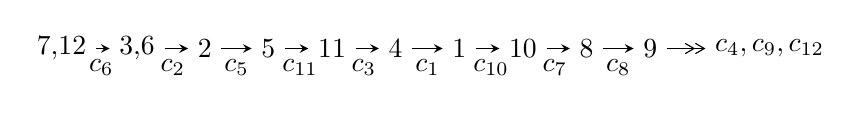
\begin{tikzpicture}[x=23pt, y=7pt]
	% node
	\node (A0) at (-1/8, 0) {7,12};
	\node (A1) at (17/16, 0) {3,6};
	\node (A2) at (17/8, 0) {2};
	\node (A3) at (25/8, 0) {5};
	\node (A4) at (33/8, 0) {11};
	\node (A5) at (41/8, 0) {4};
	\node (A6) at (49/8, 0) {1};
	\node (A7) at (57/8, 0) {10};
	\node (A8) at (65/8, 0) {8};
	\node (A9) at (73/8, 0) {9};
	\node (C1) at (1/2, -1) {$c_{6}$};
	\node (C2) at (13/8, -1) {$c_{2}$};
	\node (C3) at (21/8, -1) {$c_{5}$};
	\node (C4) at (29/8, -1) {$c_{11}$};
	\node (C5) at (37/8, -1) {$c_{3}$};
	\node (C6) at (45/8, -1) {$c_{1}$};
	\node (C7) at (53/8, -1) {$c_{10}$};
	\node (C8) at (61/8, -1) {$c_{7}$};
	\node (C9) at (69/8, -1) {$c_{8}$};
	\node (A10) at (11, 0) {$c_{4},c_{9},c_{12}$};

	% edge
	\draw[->,>=stealth]	
	(A0) edge (A1) (A1) edge (A2) (A2) edge (A3) (A3) edge (A4) (A4) edge (A5) (A5) edge (A6) (A6) edge (A7) (A7) edge (A8) (A8) edge (A9) ;
	\draw[->>,>={angle 60}]	
	(A9) edge (A10);
\end{tikzpicture} \\ 

\end{tabular} \\

\footnotetext{
The image of knot diagram is generated by the software ``\textbf{Draw programme}" developed by Andrew Bartholomew(\url{http://www.layer8.co.uk/maths/draw/index.htm\#Running-draw}), where we modified some parts for our purpose(\url{https://github.com/CATsTAILs/LinksPainter}).
}\phantom \\ \newline 
\centering \textbf{Ideals for irreducible components\footnotemark of $X_{\text{par}}$} 
 
\begin{align*}
I^u_{1}&=\langle 
3.56490\times10^{251} u^{63}+5.72448\times10^{251} u^{62}+\cdots+5.50146\times10^{254} b+8.86861\times10^{253},\\
\phantom{I^u_{1}}&\phantom{= \langle  }-2.35876\times10^{254} u^{63}-4.13220\times10^{254} u^{62}+\cdots+4.26363\times10^{255} a+8.91301\times10^{256},\\
\phantom{I^u_{1}}&\phantom{= \langle  }u^{64}+2 u^{63}+\cdots-735 u-124\rangle \\
I^u_{2}&=\langle 
284428202 u^{14}+396867456 u^{13}+\cdots+506758949 b+426150472,\\
\phantom{I^u_{2}}&\phantom{= \langle  }-8189375817 u^{14}-6846809578 u^{13}+\cdots+2533794745 a+27837731986,\\
\phantom{I^u_{2}}&\phantom{= \langle  }u^{15}+u^{14}- u^{13}+6 u^{12}+26 u^{11}+12 u^{10}-24 u^9-24 u^8-10 u^7-32 u^6+9 u^5+51 u^4+12 u^3-17 u^2-6 u-1\rangle \\
\\
\end{align*}
\raggedright * 2 irreducible components of $\dim_{\mathbb{C}}=0$, with total 79 representations.\\
\footnotetext{All coefficients of polynomials are rational numbers. But the coefficients are sometimes approximated in decimal forms when there is not enough margin.}
\newpage
\renewcommand{\arraystretch}{1}
\centering \section*{I. $I^u_{1}= \langle 3.56\times10^{251} u^{63}+5.72\times10^{251} u^{62}+\cdots+5.50\times10^{254} b+8.87\times10^{253},\;-2.36\times10^{254} u^{63}-4.13\times10^{254} u^{62}+\cdots+4.26\times10^{255} a+8.91\times10^{256},\;u^{64}+2 u^{63}+\cdots-735 u-124 \rangle$}
\flushleft \textbf{(i) Arc colorings}\\
\begin{tabular}{m{7pt} m{180pt} m{7pt} m{180pt} }
\flushright $a_{7}=$&$\begin{pmatrix}1\\0\end{pmatrix}$ \\
\flushright $a_{12}=$&$\begin{pmatrix}0\\u\end{pmatrix}$ \\
\flushright $a_{3}=$&$\begin{pmatrix}0.0553228 u^{63}+0.0969175 u^{62}+\cdots-78.2318 u-20.9047\\-0.000647992 u^{63}-0.00104054 u^{62}+\cdots-1.92857 u-0.161205\end{pmatrix}$ \\
\flushright $a_{6}=$&$\begin{pmatrix}1\\- u^2\end{pmatrix}$ \\
\flushright $a_{2}=$&$\begin{pmatrix}0.0567994 u^{63}+0.100527 u^{62}+\cdots-83.3905 u-22.7682\\-0.000281111 u^{63}-0.000325930 u^{62}+\cdots-2.59418 u-0.242607\end{pmatrix}$ \\
\flushright $a_{5}=$&$\begin{pmatrix}0.0564900 u^{63}+0.0995986 u^{62}+\cdots-85.0876 u-19.9751\\0.00255943 u^{63}+0.00450226 u^{62}+\cdots+0.805611 u+1.02426\end{pmatrix}$ \\
\flushright $a_{11}=$&$\begin{pmatrix}-0.165563 u^{63}-0.264911 u^{62}+\cdots+226.261 u+27.5914\\0.00582935 u^{63}+0.00991425 u^{62}+\cdots-9.04574 u-1.72680\end{pmatrix}$ \\
\flushright $a_{4}=$&$\begin{pmatrix}0.0723938 u^{63}-0.000941407 u^{62}+\cdots-43.1756 u+139.987\\-0.0116628 u^{63}-0.0183746 u^{62}+\cdots+13.8692 u+1.03110\end{pmatrix}$ \\
\flushright $a_{1}=$&$\begin{pmatrix}-2.03665 u^{63}-3.81811 u^{62}+\cdots+3046.36 u+1071.95\\0.0128152 u^{63}+0.0318513 u^{62}+\cdots-25.6739 u-16.6834\end{pmatrix}$ \\
\flushright $a_{10}=$&$\begin{pmatrix}-0.159734 u^{63}-0.254996 u^{62}+\cdots+217.215 u+25.8646\\0.00582935 u^{63}+0.00991425 u^{62}+\cdots-9.04574 u-1.72680\end{pmatrix}$ \\
\flushright $a_{8}=$&$\begin{pmatrix}-0.135914 u^{63}-0.259560 u^{62}+\cdots+202.668 u+78.8031\\0.00237433 u^{63}+0.00489477 u^{62}+\cdots-1.28540 u-0.718444\end{pmatrix}$ \\
\flushright $a_{9}=$&$\begin{pmatrix}2.15886 u^{63}+3.39630 u^{62}+\cdots-2926.06 u-284.022\\-0.0649284 u^{63}-0.111193 u^{62}+\cdots+97.1411 u+21.8225\end{pmatrix}$\\&\end{tabular}
\flushleft \textbf{(ii) Obstruction class $= -1$}\\~\\
\flushleft \textbf{(iii) Cusp Shapes $= 0.208334 u^{63}+0.401745 u^{62}+\cdots-321.895 u-123.850$}\\~\\
\newpage\renewcommand{\arraystretch}{1}
\flushleft \textbf{(iv) u-Polynomials at the component}\newline \\
\begin{tabular}{m{50pt}|m{274pt}}
Crossings & \hspace{64pt}u-Polynomials at each crossing \\
\hline $$\begin{aligned}c_{1}\end{aligned}$$&$\begin{aligned}
&u^{64}-5 u^{63}+\cdots+1916 u+23
\end{aligned}$\\
\hline $$\begin{aligned}c_{2},c_{5}\end{aligned}$$&$\begin{aligned}
&u^{64}+2 u^{63}+\cdots-9167 u-1601
\end{aligned}$\\
\hline $$\begin{aligned}c_{3},c_{11}\end{aligned}$$&$\begin{aligned}
&u^{64}-7 u^{63}+\cdots+229 u+41
\end{aligned}$\\
\hline $$\begin{aligned}c_{4},c_{8}\end{aligned}$$&$\begin{aligned}
&u^{64}- u^{63}+\cdots+2985 u+1949
\end{aligned}$\\
\hline $$\begin{aligned}c_{6}\end{aligned}$$&$\begin{aligned}
&u^{64}+2 u^{63}+\cdots-735 u-124
\end{aligned}$\\
\hline $$\begin{aligned}c_{7},c_{10}\end{aligned}$$&$\begin{aligned}
&u^{64}-8 u^{63}+\cdots+355 u-25
\end{aligned}$\\
\hline $$\begin{aligned}c_{9}\end{aligned}$$&$\begin{aligned}
&u^{64}+u^{63}+\cdots+8216 u-400
\end{aligned}$\\
\hline $$\begin{aligned}c_{12}\end{aligned}$$&$\begin{aligned}
&u^{64}+31 u^{63}+\cdots-13162594 u-3152393
\end{aligned}$\\
\hline
\end{tabular}\\~\\
\newpage\renewcommand{\arraystretch}{1}
\flushleft \textbf{(v) Riley Polynomials at the component}\newline \\
\begin{tabular}{m{50pt}|m{274pt}}
Crossings & \hspace{64pt}Riley Polynomials at each crossing \\
\hline $$\begin{aligned}c_{1}\end{aligned}$$&$\begin{aligned}
&y^{64}+91 y^{63}+\cdots-2472756 y+529
\end{aligned}$\\
\hline $$\begin{aligned}c_{2},c_{5}\end{aligned}$$&$\begin{aligned}
&y^{64}-36 y^{63}+\cdots-23099829 y+2563201
\end{aligned}$\\
\hline $$\begin{aligned}c_{3},c_{11}\end{aligned}$$&$\begin{aligned}
&y^{64}+41 y^{63}+\cdots+48501 y+1681
\end{aligned}$\\
\hline $$\begin{aligned}c_{4},c_{8}\end{aligned}$$&$\begin{aligned}
&y^{64}-71 y^{63}+\cdots-12929063 y+3798601
\end{aligned}$\\
\hline $$\begin{aligned}c_{6}\end{aligned}$$&$\begin{aligned}
&y^{64}-12 y^{63}+\cdots-119121 y+15376
\end{aligned}$\\
\hline $$\begin{aligned}c_{7},c_{10}\end{aligned}$$&$\begin{aligned}
&y^{64}+46 y^{63}+\cdots+6025 y+625
\end{aligned}$\\
\hline $$\begin{aligned}c_{9}\end{aligned}$$&$\begin{aligned}
&y^{64}+75 y^{63}+\cdots-82949056 y+160000
\end{aligned}$\\
\hline $$\begin{aligned}c_{12}\end{aligned}$$&$\begin{aligned}
&y^{64}-291 y^{63}+\cdots+164152624346502 y+9937581626449
\end{aligned}$\\
\hline
\end{tabular}\\~\\
\newpage\flushleft \textbf{(vi) Complex Volumes and Cusp Shapes}
$$\begin{array}{c|c|c}  
\text{Solutions to }I^u_{1}& \I (\text{vol} + \sqrt{-1}CS) & \text{Cusp shape}\\
 \hline 
\begin{aligned}
u &= -0.633361 + 0.835451 I \\
a &= -0.530837 + 1.034980 I \\
b &= -1.22852 - 1.74056 I\end{aligned}
 & \phantom{-}9.22096 + 8.60656 I & -4.00000 - 6.23706 I \\ \hline\begin{aligned}
u &= -0.633361 - 0.835451 I \\
a &= -0.530837 - 1.034980 I \\
b &= -1.22852 + 1.74056 I\end{aligned}
 & \phantom{-}9.22096 - 8.60656 I & -4.00000 + 6.23706 I \\ \hline\begin{aligned}
u &= \phantom{-}0.253229 + 0.900252 I \\
a &= \phantom{-}0.646605 - 0.735868 I \\
b &= \phantom{-}0.197400 - 0.437594 I\end{aligned}
 & \phantom{-}3.52271 + 1.68170 I & \phantom{-}3.06688 - 2.85627 I \\ \hline\begin{aligned}
u &= \phantom{-}0.253229 - 0.900252 I \\
a &= \phantom{-}0.646605 + 0.735868 I \\
b &= \phantom{-}0.197400 + 0.437594 I\end{aligned}
 & \phantom{-}3.52271 - 1.68170 I & \phantom{-}3.06688 + 2.85627 I \\ \hline\begin{aligned}
u &= -0.377573 + 0.852675 I \\
a &= \phantom{-}0.896250 - 0.658963 I \\
b &= -1.065120 + 0.904713 I\end{aligned}
 & \phantom{-}3.87587 + 2.56306 I & -0.62210 - 7.87266 I \\ \hline\begin{aligned}
u &= -0.377573 - 0.852675 I \\
a &= \phantom{-}0.896250 + 0.658963 I \\
b &= -1.065120 - 0.904713 I\end{aligned}
 & \phantom{-}3.87587 - 2.56306 I & -0.62210 + 7.87266 I \\ \hline\begin{aligned}
u &= \phantom{-}0.968214 + 0.475093 I \\
a &= \phantom{-}0.677564 - 0.491270 I \\
b &= \phantom{-}0.176332 + 0.400779 I\end{aligned}
 & \phantom{-}4.21273 - 5.33178 I & \phantom{-0.000000 } 0 \\ \hline\begin{aligned}
u &= \phantom{-}0.968214 - 0.475093 I \\
a &= \phantom{-}0.677564 + 0.491270 I \\
b &= \phantom{-}0.176332 - 0.400779 I\end{aligned}
 & \phantom{-}4.21273 + 5.33178 I & \phantom{-0.000000 } 0 \\ \hline\begin{aligned}
u &= \phantom{-}0.773876 + 0.769109 I \\
a &= \phantom{-}0.892108 - 0.775301 I \\
b &= \phantom{-}0.281562 - 0.440255 I\end{aligned}
 & \phantom{-}8.67364 - 9.43479 I & \phantom{-0.000000 } 0 \\ \hline\begin{aligned}
u &= \phantom{-}0.773876 - 0.769109 I \\
a &= \phantom{-}0.892108 + 0.775301 I \\
b &= \phantom{-}0.281562 + 0.440255 I\end{aligned}
 & \phantom{-}8.67364 + 9.43479 I & \phantom{-0.000000 } 0\\
 \hline 
 \end{array}$$\newpage$$\begin{array}{c|c|c}  
\text{Solutions to }I^u_{1}& \I (\text{vol} + \sqrt{-1}CS) & \text{Cusp shape}\\
 \hline 
\begin{aligned}
u &= -0.859282 + 0.057231 I \\
a &= -0.94062 + 1.30856 I \\
b &= -0.294118 - 0.799242 I\end{aligned}
 & \phantom{-}1.356600 - 0.236124 I & -10.20366 + 0.45727 I \\ \hline\begin{aligned}
u &= -0.859282 - 0.057231 I \\
a &= -0.94062 - 1.30856 I \\
b &= -0.294118 + 0.799242 I\end{aligned}
 & \phantom{-}1.356600 + 0.236124 I & -10.20366 - 0.45727 I \\ \hline\begin{aligned}
u &= -0.637038 + 0.946755 I \\
a &= \phantom{-}0.399510 + 0.471571 I \\
b &= \phantom{-}0.408356 + 0.442921 I\end{aligned}
 & \phantom{-}1.75404 + 3.75138 I & \phantom{-0.000000 } 0 \\ \hline\begin{aligned}
u &= -0.637038 - 0.946755 I \\
a &= \phantom{-}0.399510 - 0.471571 I \\
b &= \phantom{-}0.408356 - 0.442921 I\end{aligned}
 & \phantom{-}1.75404 - 3.75138 I & \phantom{-0.000000 } 0 \\ \hline\begin{aligned}
u &= -0.857334\phantom{ +0.000000I} \\
a &= \phantom{-}0.655331\phantom{ +0.000000I} \\
b &= \phantom{-}0.234820\phantom{ +0.000000I}\end{aligned}
 & -2.02039\phantom{ +0.000000I} & -2.98300\phantom{ +0.000000I} \\ \hline\begin{aligned}
u &= \phantom{-}0.890002 + 0.755372 I \\
a &= -0.560431 - 1.010460 I \\
b &= -0.14451 + 1.51757 I\end{aligned}
 & -5.87560 - 2.84637 I & \phantom{-0.000000 } 0 \\ \hline\begin{aligned}
u &= \phantom{-}0.890002 - 0.755372 I \\
a &= -0.560431 + 1.010460 I \\
b &= -0.14451 - 1.51757 I\end{aligned}
 & -5.87560 + 2.84637 I & \phantom{-0.000000 } 0 \\ \hline\begin{aligned}
u &= -0.905414 + 0.761217 I \\
a &= \phantom{-}0.319731 - 0.980710 I \\
b &= \phantom{-}1.01703 + 1.40700 I\end{aligned}
 & \phantom{-}1.05509 + 3.06315 I & \phantom{-0.000000 } 0 \\ \hline\begin{aligned}
u &= -0.905414 - 0.761217 I \\
a &= \phantom{-}0.319731 + 0.980710 I \\
b &= \phantom{-}1.01703 - 1.40700 I\end{aligned}
 & \phantom{-}1.05509 - 3.06315 I & \phantom{-0.000000 } 0 \\ \hline\begin{aligned}
u &= \phantom{-}0.629031 + 0.441968 I \\
a &= -0.590354 - 1.251080 I \\
b &= -1.30236 + 1.41946 I\end{aligned}
 & -0.87655 - 3.21386 I & -5.46121 + 1.99366 I\\
 \hline 
 \end{array}$$\newpage$$\begin{array}{c|c|c}  
\text{Solutions to }I^u_{1}& \I (\text{vol} + \sqrt{-1}CS) & \text{Cusp shape}\\
 \hline 
\begin{aligned}
u &= \phantom{-}0.629031 - 0.441968 I \\
a &= -0.590354 + 1.251080 I \\
b &= -1.30236 - 1.41946 I\end{aligned}
 & -0.87655 + 3.21386 I & -5.46121 - 1.99366 I \\ \hline\begin{aligned}
u &= \phantom{-}0.745958\phantom{ +0.000000I} \\
a &= -0.843570\phantom{ +0.000000I} \\
b &= -0.794982\phantom{ +0.000000I}\end{aligned}
 & -2.75005\phantom{ +0.000000I} & \phantom{-}2.80630\phantom{ +0.000000I} \\ \hline\begin{aligned}
u &= \phantom{-}0.325605 + 1.226800 I \\
a &= -0.479590 + 0.579451 I \\
b &= \phantom{-}0.135918 + 0.142703 I\end{aligned}
 & \phantom{-}11.41820 - 3.52473 I & \phantom{-0.000000 } 0 \\ \hline\begin{aligned}
u &= \phantom{-}0.325605 - 1.226800 I \\
a &= -0.479590 - 0.579451 I \\
b &= \phantom{-}0.135918 - 0.142703 I\end{aligned}
 & \phantom{-}11.41820 + 3.52473 I & \phantom{-0.000000 } 0 \\ \hline\begin{aligned}
u &= \phantom{-}0.499154 + 0.523034 I \\
a &= -0.352111 - 0.051255 I \\
b &= \phantom{-}0.811508 - 0.885581 I\end{aligned}
 & \phantom{-}5.67586 + 1.02167 I & \phantom{-}0.667278 + 0.621622 I \\ \hline\begin{aligned}
u &= \phantom{-}0.499154 - 0.523034 I \\
a &= -0.352111 + 0.051255 I \\
b &= \phantom{-}0.811508 + 0.885581 I\end{aligned}
 & \phantom{-}5.67586 - 1.02167 I & \phantom{-}0.667278 - 0.621622 I \\ \hline\begin{aligned}
u &= \phantom{-}1.233920 + 0.559467 I \\
a &= \phantom{-}0.154791 + 0.866376 I \\
b &= -0.10145 - 1.88879 I\end{aligned}
 & -5.32904 - 3.11782 I & \phantom{-0.000000 } 0 \\ \hline\begin{aligned}
u &= \phantom{-}1.233920 - 0.559467 I \\
a &= \phantom{-}0.154791 - 0.866376 I \\
b &= -0.10145 + 1.88879 I\end{aligned}
 & -5.32904 + 3.11782 I & \phantom{-0.000000 } 0 \\ \hline\begin{aligned}
u &= -0.666405 + 1.183570 I \\
a &= \phantom{-}0.923395 - 0.459675 I \\
b &= \phantom{-}0.647996 + 0.764798 I\end{aligned}
 & \phantom{-}1.02762 - 2.42841 I & \phantom{-0.000000 } 0 \\ \hline\begin{aligned}
u &= -0.666405 - 1.183570 I \\
a &= \phantom{-}0.923395 + 0.459675 I \\
b &= \phantom{-}0.647996 - 0.764798 I\end{aligned}
 & \phantom{-}1.02762 + 2.42841 I & \phantom{-0.000000 } 0\\
 \hline 
 \end{array}$$\newpage$$\begin{array}{c|c|c}  
\text{Solutions to }I^u_{1}& \I (\text{vol} + \sqrt{-1}CS) & \text{Cusp shape}\\
 \hline 
\begin{aligned}
u &= \phantom{-}1.113490 + 0.809533 I \\
a &= -0.233838 - 1.094600 I \\
b &= -0.77959 + 1.53834 I\end{aligned}
 & -2.47783 - 8.59651 I & \phantom{-0.000000 } 0 \\ \hline\begin{aligned}
u &= \phantom{-}1.113490 - 0.809533 I \\
a &= -0.233838 + 1.094600 I \\
b &= -0.77959 - 1.53834 I\end{aligned}
 & -2.47783 + 8.59651 I & \phantom{-0.000000 } 0 \\ \hline\begin{aligned}
u &= -0.604799 + 0.139734 I \\
a &= \phantom{-}0.485635 - 1.204360 I \\
b &= -0.556677 + 0.966102 I\end{aligned}
 & -0.236047 + 0.888762 I & -5.62676 - 4.10196 I \\ \hline\begin{aligned}
u &= -0.604799 - 0.139734 I \\
a &= \phantom{-}0.485635 + 1.204360 I \\
b &= -0.556677 - 0.966102 I\end{aligned}
 & -0.236047 - 0.888762 I & -5.62676 + 4.10196 I \\ \hline\begin{aligned}
u &= \phantom{-}0.607795 + 0.087221 I \\
a &= -0.74621 - 1.56542 I \\
b &= \phantom{-}0.68831 + 1.51458 I\end{aligned}
 & -0.88330 + 3.97137 I & -1.334301 - 0.429545 I \\ \hline\begin{aligned}
u &= \phantom{-}0.607795 - 0.087221 I \\
a &= -0.74621 + 1.56542 I \\
b &= \phantom{-}0.68831 - 1.51458 I\end{aligned}
 & -0.88330 - 3.97137 I & -1.334301 + 0.429545 I \\ \hline\begin{aligned}
u &= \phantom{-}0.329116 + 0.508643 I \\
a &= -0.34712 + 2.17987 I \\
b &= -0.460457 + 0.282285 I\end{aligned}
 & \phantom{-}0.391230 - 0.353831 I & -2.98869 - 0.49409 I \\ \hline\begin{aligned}
u &= \phantom{-}0.329116 - 0.508643 I \\
a &= -0.34712 - 2.17987 I \\
b &= -0.460457 - 0.282285 I\end{aligned}
 & \phantom{-}0.391230 + 0.353831 I & -2.98869 + 0.49409 I \\ \hline\begin{aligned}
u &= -1.14937 + 0.90634 I \\
a &= -0.347312 + 0.828119 I \\
b &= -0.076957 - 1.360690 I\end{aligned}
 & -6.72812 + 3.57989 I & \phantom{-0.000000 } 0 \\ \hline\begin{aligned}
u &= -1.14937 - 0.90634 I \\
a &= -0.347312 - 0.828119 I \\
b &= -0.076957 + 1.360690 I\end{aligned}
 & -6.72812 - 3.57989 I & \phantom{-0.000000 } 0\\
 \hline 
 \end{array}$$\newpage$$\begin{array}{c|c|c}  
\text{Solutions to }I^u_{1}& \I (\text{vol} + \sqrt{-1}CS) & \text{Cusp shape}\\
 \hline 
\begin{aligned}
u &= -0.02527 + 1.46729 I \\
a &= -0.603836 + 0.026259 I \\
b &= \phantom{-}0.038716 + 0.193115 I\end{aligned}
 & \phantom{-}0.33931 + 2.46518 I & \phantom{-0.000000 } 0 \\ \hline\begin{aligned}
u &= -0.02527 - 1.46729 I \\
a &= -0.603836 - 0.026259 I \\
b &= \phantom{-}0.038716 - 0.193115 I\end{aligned}
 & \phantom{-}0.33931 - 2.46518 I & \phantom{-0.000000 } 0 \\ \hline\begin{aligned}
u &= -1.15018 + 0.95185 I \\
a &= \phantom{-}0.338925 - 0.857634 I \\
b &= \phantom{-}0.21681 + 1.86662 I\end{aligned}
 & -0.23323 + 9.95941 I & \phantom{-0.000000 } 0 \\ \hline\begin{aligned}
u &= -1.15018 - 0.95185 I \\
a &= \phantom{-}0.338925 + 0.857634 I \\
b &= \phantom{-}0.21681 - 1.86662 I\end{aligned}
 & -0.23323 - 9.95941 I & \phantom{-0.000000 } 0 \\ \hline\begin{aligned}
u &= -0.373052 + 0.273303 I \\
a &= \phantom{-}0.467221 - 1.081940 I \\
b &= -0.213074 + 0.512505 I\end{aligned}
 & -0.286450 + 0.969073 I & -5.20156 - 6.74642 I \\ \hline\begin{aligned}
u &= -0.373052 - 0.273303 I \\
a &= \phantom{-}0.467221 + 1.081940 I \\
b &= -0.213074 - 0.512505 I\end{aligned}
 & -0.286450 - 0.969073 I & -5.20156 + 6.74642 I \\ \hline\begin{aligned}
u &= -0.064752 + 0.327363 I \\
a &= -2.26682 + 0.73356 I \\
b &= \phantom{-}0.76192 - 1.90756 I\end{aligned}
 & \phantom{-}5.41696 + 1.08390 I & \phantom{-}7.59845 - 2.56360 I \\ \hline\begin{aligned}
u &= -0.064752 - 0.327363 I \\
a &= -2.26682 - 0.73356 I \\
b &= \phantom{-}0.76192 + 1.90756 I\end{aligned}
 & \phantom{-}5.41696 - 1.08390 I & \phantom{-}7.59845 + 2.56360 I \\ \hline\begin{aligned}
u &= -0.264144 + 0.158619 I \\
a &= -2.22385 - 11.81440 I \\
b &= \phantom{-}0.174020 + 0.255284 I\end{aligned}
 & \phantom{-}1.84425 - 0.21555 I & -54.1683 - 39.7304 I \\ \hline\begin{aligned}
u &= -0.264144 - 0.158619 I \\
a &= -2.22385 + 11.81440 I \\
b &= \phantom{-}0.174020 - 0.255284 I\end{aligned}
 & \phantom{-}1.84425 + 0.21555 I & -54.1683 + 39.7304 I\\
 \hline 
 \end{array}$$\newpage$$\begin{array}{c|c|c}  
\text{Solutions to }I^u_{1}& \I (\text{vol} + \sqrt{-1}CS) & \text{Cusp shape}\\
 \hline 
\begin{aligned}
u &= -1.51312 + 1.02719 I \\
a &= -0.147229 + 0.787597 I \\
b &= -0.85869 - 1.71762 I\end{aligned}
 & -4.27079 + 6.80776 I & \phantom{-0.000000 } 0 \\ \hline\begin{aligned}
u &= -1.51312 - 1.02719 I \\
a &= -0.147229 - 0.787597 I \\
b &= -0.85869 + 1.71762 I\end{aligned}
 & -4.27079 - 6.80776 I & \phantom{-0.000000 } 0 \\ \hline\begin{aligned}
u &= -1.42579 + 1.18878 I \\
a &= \phantom{-}0.215991 - 0.781332 I \\
b &= \phantom{-}1.04536 + 1.90254 I\end{aligned}
 & \phantom{-}4.6282 + 16.0012 I & \phantom{-0.000000 } 0 \\ \hline\begin{aligned}
u &= -1.42579 - 1.18878 I \\
a &= \phantom{-}0.215991 + 0.781332 I \\
b &= \phantom{-}1.04536 - 1.90254 I\end{aligned}
 & \phantom{-}4.6282 - 16.0012 I & \phantom{-0.000000 } 0 \\ \hline\begin{aligned}
u &= \phantom{-}1.89889 + 0.04609 I \\
a &= \phantom{-}0.259481 + 0.412233 I \\
b &= \phantom{-}0.01829 - 2.23354 I\end{aligned}
 & \phantom{-}6.42656 + 2.16286 I & \phantom{-0.000000 } 0 \\ \hline\begin{aligned}
u &= \phantom{-}1.89889 - 0.04609 I \\
a &= \phantom{-}0.259481 - 0.412233 I \\
b &= \phantom{-}0.01829 + 2.23354 I\end{aligned}
 & \phantom{-}6.42656 - 2.16286 I & \phantom{-0.000000 } 0 \\ \hline\begin{aligned}
u &= \phantom{-}1.64927 + 1.03875 I \\
a &= \phantom{-}0.137830 + 0.664791 I \\
b &= \phantom{-}1.06970 - 2.10818 I\end{aligned}
 & -1.72416 - 8.22153 I & \phantom{-0.000000 } 0 \\ \hline\begin{aligned}
u &= \phantom{-}1.64927 - 1.03875 I \\
a &= \phantom{-}0.137830 - 0.664791 I \\
b &= \phantom{-}1.06970 + 2.10818 I\end{aligned}
 & -1.72416 + 8.22153 I & \phantom{-0.000000 } 0 \\ \hline\begin{aligned}
u &= \phantom{-}1.71347 + 1.01637 I \\
a &= \phantom{-}0.168962 + 0.420273 I \\
b &= \phantom{-}2.00584 - 2.12827 I\end{aligned}
 & \phantom{-}6.48830 + 3.36563 I & \phantom{-0.000000 } 0 \\ \hline\begin{aligned}
u &= \phantom{-}1.71347 - 1.01637 I \\
a &= \phantom{-}0.168962 - 0.420273 I \\
b &= \phantom{-}2.00584 + 2.12827 I\end{aligned}
 & \phantom{-}6.48830 - 3.36563 I & \phantom{-0.000000 } 0\\
 \hline 
 \end{array}$$\newpage$$\begin{array}{c|c|c}  
\text{Solutions to }I^u_{1}& \I (\text{vol} + \sqrt{-1}CS) & \text{Cusp shape}\\
 \hline 
\begin{aligned}
u &= -1.85043 + 0.96309 I \\
a &= -0.431038 + 0.249730 I \\
b &= -0.75543 - 1.82108 I\end{aligned}
 & \phantom{-}6.12807 - 2.09855 I & \phantom{-0.000000 } 0 \\ \hline\begin{aligned}
u &= -1.85043 - 0.96309 I \\
a &= -0.431038 - 0.249730 I \\
b &= -0.75543 + 1.82108 I\end{aligned}
 & \phantom{-}6.12807 + 2.09855 I & \phantom{-0.000000 } 0 \\ \hline\begin{aligned}
u &= -1.32939 + 2.57903 I \\
a &= \phantom{-}0.318575 - 0.116709 I \\
b &= \phantom{-}1.42196 + 1.34450 I\end{aligned}
 & \phantom{-}6.24532 - 4.56303 I & \phantom{-0.000000 } 0 \\ \hline\begin{aligned}
u &= -1.32939 - 2.57903 I \\
a &= \phantom{-}0.318575 + 0.116709 I \\
b &= \phantom{-}1.42196 - 1.34450 I\end{aligned}
 & \phantom{-}6.24532 + 4.56303 I & \phantom{-0.000000 } 0\\
 \hline 
 \end{array}$$\newpage\newpage\renewcommand{\arraystretch}{1}
\centering \section*{II. $I^u_{2}= \langle 2.84\times10^{8} u^{14}+3.97\times10^{8} u^{13}+\cdots+5.07\times10^{8} b+4.26\times10^{8},\;-8.19\times10^{9} u^{14}-6.85\times10^{9} u^{13}+\cdots+2.53\times10^{9} a+2.78\times10^{10},\;u^{15}+u^{14}+\cdots-6 u-1 \rangle$}
\flushleft \textbf{(i) Arc colorings}\\
\begin{tabular}{m{7pt} m{180pt} m{7pt} m{180pt} }
\flushright $a_{7}=$&$\begin{pmatrix}1\\0\end{pmatrix}$ \\
\flushright $a_{12}=$&$\begin{pmatrix}0\\u\end{pmatrix}$ \\
\flushright $a_{3}=$&$\begin{pmatrix}3.23206 u^{14}+2.70220 u^{13}+\cdots-61.4746 u-10.9866\\-0.561269 u^{14}-0.783148 u^{13}+\cdots-4.05570 u-0.840933\end{pmatrix}$ \\
\flushright $a_{6}=$&$\begin{pmatrix}1\\- u^2\end{pmatrix}$ \\
\flushright $a_{2}=$&$\begin{pmatrix}2.65780 u^{14}+1.80378 u^{13}+\cdots-65.4774 u-12.3574\\-0.119451 u^{14}-0.0902996 u^{13}+\cdots-1.53653 u-0.516781\end{pmatrix}$ \\
\flushright $a_{5}=$&$\begin{pmatrix}2.70220 u^{14}+2.15934 u^{13}+\cdots-53.0688 u-7.75452\\0.0495199 u^{14}+0.0757808 u^{13}+\cdots+0.0115506 u-0.198240\end{pmatrix}$ \\
\flushright $a_{11}=$&$\begin{pmatrix}-6.42929 u^{14}-4.92808 u^{13}+\cdots+115.242 u+4.54807\\-0.125520 u^{14}+0.0522556 u^{13}+\cdots+7.01627 u+1.26673\end{pmatrix}$ \\
\flushright $a_{4}=$&$\begin{pmatrix}7.05889 u^{14}+2.95931 u^{13}+\cdots-126.691 u+32.5632\\0.412693 u^{14}+0.120412 u^{13}+\cdots-13.9640 u-1.29863\end{pmatrix}$ \\
\flushright $a_{1}=$&$\begin{pmatrix}-16.6301 u^{14}-19.6871 u^{13}+\cdots+325.929 u+144.504\\0.000494896 u^{14}-0.495565 u^{13}+\cdots-7.85539 u+2.68332\end{pmatrix}$ \\
\flushright $a_{10}=$&$\begin{pmatrix}-6.55481 u^{14}-4.87583 u^{13}+\cdots+122.258 u+5.81480\\-0.125520 u^{14}+0.0522556 u^{13}+\cdots+7.01627 u+1.26673\end{pmatrix}$ \\
\flushright $a_{8}=$&$\begin{pmatrix}4.05411 u^{14}+4.62887 u^{13}+\cdots-73.3182 u-29.1773\\0.264042 u^{14}+0.287559 u^{13}+\cdots+2.00556 u-0.550328\end{pmatrix}$ \\
\flushright $a_{9}=$&$\begin{pmatrix}-39.5909 u^{14}-29.6382 u^{13}+\cdots+741.709 u+48.4775\\-1.18765 u^{14}-0.793252 u^{13}+\cdots+35.0448 u+6.68072\end{pmatrix}$\\&\end{tabular}
\flushleft \textbf{(ii) Obstruction class $= 1$}\\~\\
\flushleft \textbf{(iii) Cusp Shapes $= -\frac{6764270976}{2533794745} u^{14}-\frac{13464586804}{2533794745} u^{13}+\cdots+\frac{54402764179}{2533794745} u+\frac{37139257588}{2533794745}$}\\~\\
\newpage\renewcommand{\arraystretch}{1}
\flushleft \textbf{(iv) u-Polynomials at the component}\newline \\
\begin{tabular}{m{50pt}|m{274pt}}
Crossings & \hspace{64pt}u-Polynomials at each crossing \\
\hline $$\begin{aligned}c_{1}\end{aligned}$$&$\begin{aligned}
&u^{15}+4 u^{14}+\cdots+31 u-11
\end{aligned}$\\
\hline $$\begin{aligned}c_{2}\end{aligned}$$&$\begin{aligned}
&u^{15}+5 u^{14}+\cdots-12 u-9
\end{aligned}$\\
\hline $$\begin{aligned}c_{3}\end{aligned}$$&$\begin{aligned}
&u^{15}-2 u^{14}+\cdots+2 u+1
\end{aligned}$\\
\hline $$\begin{aligned}c_{4}\end{aligned}$$&$\begin{aligned}
&u^{15}+4 u^{14}+\cdots+5 u^2-1
\end{aligned}$\\
\hline $$\begin{aligned}c_{5}\end{aligned}$$&$\begin{aligned}
&u^{15}-5 u^{14}+\cdots-12 u+9
\end{aligned}$\\
\hline $$\begin{aligned}c_{6}\end{aligned}$$&$\begin{aligned}
&u^{15}+u^{14}+\cdots-6 u-1
\end{aligned}$\\
\hline $$\begin{aligned}c_{7}\end{aligned}$$&$\begin{aligned}
&u^{15}-3 u^{14}+\cdots+30 u-7
\end{aligned}$\\
\hline $$\begin{aligned}c_{8}\end{aligned}$$&$\begin{aligned}
&u^{15}-4 u^{14}+\cdots-5 u^2+1
\end{aligned}$\\
\hline $$\begin{aligned}c_{9}\end{aligned}$$&$\begin{aligned}
&u^{15}+6 u^{13}+\cdots+3 u-1
\end{aligned}$\\
\hline $$\begin{aligned}c_{10}\end{aligned}$$&$\begin{aligned}
&u^{15}+3 u^{14}+\cdots+30 u+7
\end{aligned}$\\
\hline $$\begin{aligned}c_{11}\end{aligned}$$&$\begin{aligned}
&u^{15}+2 u^{14}+\cdots+2 u-1
\end{aligned}$\\
\hline $$\begin{aligned}c_{12}\end{aligned}$$&$\begin{aligned}
&u^{15}+10 u^{14}+\cdots+21 u+9
\end{aligned}$\\
\hline
\end{tabular}\\~\\
\newpage\renewcommand{\arraystretch}{1}
\flushleft \textbf{(v) Riley Polynomials at the component}\newline \\
\begin{tabular}{m{50pt}|m{274pt}}
Crossings & \hspace{64pt}Riley Polynomials at each crossing \\
\hline $$\begin{aligned}c_{1}\end{aligned}$$&$\begin{aligned}
&y^{15}+8 y^{14}+\cdots-29 y-121
\end{aligned}$\\
\hline $$\begin{aligned}c_{2},c_{5}\end{aligned}$$&$\begin{aligned}
&y^{15}-11 y^{14}+\cdots+504 y-81
\end{aligned}$\\
\hline $$\begin{aligned}c_{3},c_{11}\end{aligned}$$&$\begin{aligned}
&y^{15}+10 y^{14}+\cdots-14 y-1
\end{aligned}$\\
\hline $$\begin{aligned}c_{4},c_{8}\end{aligned}$$&$\begin{aligned}
&y^{15}-6 y^{14}+\cdots+10 y-1
\end{aligned}$\\
\hline $$\begin{aligned}c_{6}\end{aligned}$$&$\begin{aligned}
&y^{15}-3 y^{14}+\cdots+2 y-1
\end{aligned}$\\
\hline $$\begin{aligned}c_{7},c_{10}\end{aligned}$$&$\begin{aligned}
&y^{15}+11 y^{14}+\cdots-10 y-49
\end{aligned}$\\
\hline $$\begin{aligned}c_{9}\end{aligned}$$&$\begin{aligned}
&y^{15}+12 y^{14}+\cdots+11 y-1
\end{aligned}$\\
\hline $$\begin{aligned}c_{12}\end{aligned}$$&$\begin{aligned}
&y^{15}-46 y^{14}+\cdots+153 y-81
\end{aligned}$\\
\hline
\end{tabular}\\~\\
\newpage\flushleft \textbf{(vi) Complex Volumes and Cusp Shapes}
$$\begin{array}{c|c|c}  
\text{Solutions to }I^u_{2}& \I (\text{vol} + \sqrt{-1}CS) & \text{Cusp shape}\\
 \hline 
\begin{aligned}
u &= \phantom{-}0.210934 + 1.069980 I \\
a &= \phantom{-}0.349370 + 0.185058 I \\
b &= -0.648553 + 0.253657 I\end{aligned}
 & \phantom{-}1.22966 - 2.43908 I & -0.15311 + 1.71479 I \\ \hline\begin{aligned}
u &= \phantom{-}0.210934 - 1.069980 I \\
a &= \phantom{-}0.349370 - 0.185058 I \\
b &= -0.648553 - 0.253657 I\end{aligned}
 & \phantom{-}1.22966 + 2.43908 I & -0.15311 - 1.71479 I \\ \hline\begin{aligned}
u &= \phantom{-}0.884019 + 0.098357 I \\
a &= -0.056574 - 0.974530 I \\
b &= \phantom{-}1.08511 + 2.03952 I\end{aligned}
 & \phantom{-}4.78310 - 1.20532 I & -6.85327 + 1.75712 I \\ \hline\begin{aligned}
u &= \phantom{-}0.884019 - 0.098357 I \\
a &= -0.056574 + 0.974530 I \\
b &= \phantom{-}1.08511 - 2.03952 I\end{aligned}
 & \phantom{-}4.78310 + 1.20532 I & -6.85327 - 1.75712 I \\ \hline\begin{aligned}
u &= \phantom{-}0.875489\phantom{ +0.000000I} \\
a &= -0.596402\phantom{ +0.000000I} \\
b &= -0.730423\phantom{ +0.000000I}\end{aligned}
 & -3.25365\phantom{ +0.000000I} & -14.4510\phantom{ +0.000000I} \\ \hline\begin{aligned}
u &= -0.772671 + 0.267375 I \\
a &= \phantom{-}0.109162 - 1.363130 I \\
b &= \phantom{-}0.90057 + 1.67261 I\end{aligned}
 & -1.41494 + 4.47917 I & -9.52176 - 8.69041 I \\ \hline\begin{aligned}
u &= -0.772671 - 0.267375 I \\
a &= \phantom{-}0.109162 + 1.363130 I \\
b &= \phantom{-}0.90057 - 1.67261 I\end{aligned}
 & -1.41494 - 4.47917 I & -9.52176 + 8.69041 I \\ \hline\begin{aligned}
u &= -1.111680 + 0.803082 I \\
a &= -0.366596 + 0.898410 I \\
b &= \phantom{-}0.02909 - 1.54137 I\end{aligned}
 & -7.54522 + 3.13534 I & -12.90276 - 1.18531 I \\ \hline\begin{aligned}
u &= -1.111680 - 0.803082 I \\
a &= -0.366596 - 0.898410 I \\
b &= \phantom{-}0.02909 + 1.54137 I\end{aligned}
 & -7.54522 - 3.13534 I & -12.90276 + 1.18531 I \\ \hline\begin{aligned}
u &= -1.50791 + 0.90732 I \\
a &= -0.118198 + 0.835276 I \\
b &= -0.80441 - 1.75992 I\end{aligned}
 & -4.71766 + 7.82049 I & -7.90270 - 7.21830 I\\
 \hline 
 \end{array}$$\newpage$$\begin{array}{c|c|c}  
\text{Solutions to }I^u_{2}& \I (\text{vol} + \sqrt{-1}CS) & \text{Cusp shape}\\
 \hline 
\begin{aligned}
u &= -1.50791 - 0.90732 I \\
a &= -0.118198 - 0.835276 I \\
b &= -0.80441 + 1.75992 I\end{aligned}
 & -4.71766 - 7.82049 I & -7.90270 + 7.21830 I \\ \hline\begin{aligned}
u &= -0.157840 + 0.171948 I \\
a &= \phantom{-}0.10064 - 10.05960 I \\
b &= -0.272890 - 0.178968 I\end{aligned}
 & \phantom{-}1.94655 - 0.28740 I & \phantom{-}10.27253 + 8.40570 I \\ \hline\begin{aligned}
u &= -0.157840 - 0.171948 I \\
a &= \phantom{-}0.10064 + 10.05960 I \\
b &= -0.272890 + 0.178968 I\end{aligned}
 & \phantom{-}1.94655 + 0.28740 I & \phantom{-}10.27253 - 8.40570 I \\ \hline\begin{aligned}
u &= \phantom{-}1.51740 + 1.84920 I \\
a &= \phantom{-}0.280397 + 0.100742 I \\
b &= \phantom{-}1.57630 - 1.96372 I\end{aligned}
 & \phantom{-}7.34533 + 4.44406 I & \phantom{-}3.28670 - 5.71136 I \\ \hline\begin{aligned}
u &= \phantom{-}1.51740 - 1.84920 I \\
a &= \phantom{-}0.280397 - 0.100742 I \\
b &= \phantom{-}1.57630 + 1.96372 I\end{aligned}
 & \phantom{-}7.34533 - 4.44406 I & \phantom{-}3.28670 + 5.71136 I\\
 \hline 
 \end{array}$$\newpage
\newpage\renewcommand{\arraystretch}{1}
\centering \section*{ III. u-Polynomials}
\begin{tabular}{m{50pt}|m{274pt}}
Crossings & \hspace{64pt}u-Polynomials at each crossing \\
\hline $$\begin{aligned}c_{1}\end{aligned}$$&$\begin{aligned}
&(u^{15}+4 u^{14}+\cdots+31 u-11)(u^{64}-5 u^{63}+\cdots+1916 u+23)
\end{aligned}$\\
\hline $$\begin{aligned}c_{2}\end{aligned}$$&$\begin{aligned}
&(u^{15}+5 u^{14}+\cdots-12 u-9)(u^{64}+2 u^{63}+\cdots-9167 u-1601)
\end{aligned}$\\
\hline $$\begin{aligned}c_{3}\end{aligned}$$&$\begin{aligned}
&(u^{15}-2 u^{14}+\cdots+2 u+1)(u^{64}-7 u^{63}+\cdots+229 u+41)
\end{aligned}$\\
\hline $$\begin{aligned}c_{4}\end{aligned}$$&$\begin{aligned}
&(u^{15}+4 u^{14}+\cdots+5 u^2-1)(u^{64}- u^{63}+\cdots+2985 u+1949)
\end{aligned}$\\
\hline $$\begin{aligned}c_{5}\end{aligned}$$&$\begin{aligned}
&(u^{15}-5 u^{14}+\cdots-12 u+9)(u^{64}+2 u^{63}+\cdots-9167 u-1601)
\end{aligned}$\\
\hline $$\begin{aligned}c_{6}\end{aligned}$$&$\begin{aligned}
&(u^{15}+u^{14}+\cdots-6 u-1)(u^{64}+2 u^{63}+\cdots-735 u-124)
\end{aligned}$\\
\hline $$\begin{aligned}c_{7}\end{aligned}$$&$\begin{aligned}
&(u^{15}-3 u^{14}+\cdots+30 u-7)(u^{64}-8 u^{63}+\cdots+355 u-25)
\end{aligned}$\\
\hline $$\begin{aligned}c_{8}\end{aligned}$$&$\begin{aligned}
&(u^{15}-4 u^{14}+\cdots-5 u^2+1)(u^{64}- u^{63}+\cdots+2985 u+1949)
\end{aligned}$\\
\hline $$\begin{aligned}c_{9}\end{aligned}$$&$\begin{aligned}
&(u^{15}+6 u^{13}+\cdots+3 u-1)(u^{64}+u^{63}+\cdots+8216 u-400)
\end{aligned}$\\
\hline $$\begin{aligned}c_{10}\end{aligned}$$&$\begin{aligned}
&(u^{15}+3 u^{14}+\cdots+30 u+7)(u^{64}-8 u^{63}+\cdots+355 u-25)
\end{aligned}$\\
\hline $$\begin{aligned}c_{11}\end{aligned}$$&$\begin{aligned}
&(u^{15}+2 u^{14}+\cdots+2 u-1)(u^{64}-7 u^{63}+\cdots+229 u+41)
\end{aligned}$\\
\hline $$\begin{aligned}c_{12}\end{aligned}$$&$\begin{aligned}
&(u^{15}+10 u^{14}+\cdots+21 u+9)\\
&\cdot(u^{64}+31 u^{63}+\cdots-13162594 u-3152393)
\end{aligned}$\\
\hline
\end{tabular}\newpage\renewcommand{\arraystretch}{1}
\centering \section*{ IV. Riley Polynomials}
\begin{tabular}{m{50pt}|m{274pt}}
Crossings & \hspace{64pt}Riley Polynomials at each crossing \\
\hline $$\begin{aligned}c_{1}\end{aligned}$$&$\begin{aligned}
&(y^{15}+8 y^{14}+\cdots-29 y-121)(y^{64}+91 y^{63}+\cdots-2472756 y+529)
\end{aligned}$\\
\hline $$\begin{aligned}c_{2},c_{5}\end{aligned}$$&$\begin{aligned}
&(y^{15}-11 y^{14}+\cdots+504 y-81)\\
&\cdot(y^{64}-36 y^{63}+\cdots-23099829 y+2563201)
\end{aligned}$\\
\hline $$\begin{aligned}c_{3},c_{11}\end{aligned}$$&$\begin{aligned}
&(y^{15}+10 y^{14}+\cdots-14 y-1)(y^{64}+41 y^{63}+\cdots+48501 y+1681)
\end{aligned}$\\
\hline $$\begin{aligned}c_{4},c_{8}\end{aligned}$$&$\begin{aligned}
&(y^{15}-6 y^{14}+\cdots+10 y-1)\\
&\cdot(y^{64}-71 y^{63}+\cdots-12929063 y+3798601)
\end{aligned}$\\
\hline $$\begin{aligned}c_{6}\end{aligned}$$&$\begin{aligned}
&(y^{15}-3 y^{14}+\cdots+2 y-1)(y^{64}-12 y^{63}+\cdots-119121 y+15376)
\end{aligned}$\\
\hline $$\begin{aligned}c_{7},c_{10}\end{aligned}$$&$\begin{aligned}
&(y^{15}+11 y^{14}+\cdots-10 y-49)(y^{64}+46 y^{63}+\cdots+6025 y+625)
\end{aligned}$\\
\hline $$\begin{aligned}c_{9}\end{aligned}$$&$\begin{aligned}
&(y^{15}+12 y^{14}+\cdots+11 y-1)\\
&\cdot(y^{64}+75 y^{63}+\cdots-82949056 y+160000)
\end{aligned}$\\
\hline $$\begin{aligned}c_{12}\end{aligned}$$&$\begin{aligned}
&(y^{15}-46 y^{14}+\cdots+153 y-81)\\
&\cdot(y^{64}-291 y^{63}+\cdots+164152624346502 y+9937581626449)
\end{aligned}$\\
\hline
\end{tabular}
\vskip 2pc
\end{document}